\chapter{Background}
\section{Homomorphic Encryption}
Homomorphic encryption is a form of encryption that allows computations to be performed on ciphertexts, thus generating an encrypted result, which when decrypted matches the result of operations performed on the plaintext. For example, the numbers 4 and 5 could be encrypted to \verb|A| and \verb|B|. Let \verb|C| = \verb|A| $+$ \verb|B|. When \verb|C| is decrypted, its value will be 9. So common operations, like addition and multiplication, can be performed on encrypted data, and produce the same result as if the data was not encrypted in the first place. This is a desired feature in encryption schemes, because it allows encrypted data to be passed from online service to online service, each service performing operations on the data, without the online service knowing what the data is. 

Currently, for an online service to perform an operation for a user, the online service must know what the data is. Thus any online service will know what data a user is giving them. However with homomorphic encryption, an online service (even an untrusted online service), can perform operations on user data, without the user being worried about their data being known or exposed. 

A fully homomorphic encryption (FHE) scheme has long been sought after \cite{rivest1978data}. For a scheme to be fully homomorphic, any arbitrary operation must be able to be executed, and still produce the correct results. It may seem like many operations need to be supported if any arbitrary operation can be performed, but in reality a fully homomorphic scheme need only support both addition and multiplication, as every other operation can be derived from those two. Partially homomorphic encryption schemes, schemes that only support one operation, have been known to exist since the 1970s. A few schemes that are known to be partially homomorphic are Unpadded RSA, ElGamal, Goldwasser-Micali, Benaloh, and Paillier. All of these schemes only support one operation, either addition or multiplication, but not both. It took more than 30 years before a fully homomorphic scheme was designed by Craig Gentry.

\subsection{Gentry's Design}
Craig Gentry proposed the first fully homomorphic encryption scheme in 2009 utilizing lattice-based cryptography \cite{gentry2009fully}. His scheme supported both addition and multiplication, from which any arbitrary operation could be derived. 

Gentry started by designing what was called a somewhat homomorphic encryption (SWHE) scheme. A SWHE scheme supports arbitrary operations, but could only compute a limited number of operations. This is because the scheme uses a noise factor when representing a ciphertext. When an operation is performed the noise in the representation grows. If the noise grows too large, then the ciphertext becomes incorrect when decrypted. Gentry then took this SWHE scheme and added bootstrapping, meaning it could evaluate its own decryption circuit. This bootstrapping procedure allowed for the cipthertexts to be \say{refreshed}, where the noise would be decreased, thus allowing for more operations to take place. Finally Gentry proved that a bootstrappable SWHE scheme can be made into a FHE scheme, by continually performing the bootstrapping procedure when the noise reaches a certain limit.

Gentry's scheme was the first construction of a FHE scheme, however impractical when implemented \cite{cryptoeprint:2010:520}, because the ciphertext size and computation time increased sharply as the security level increased. It could take upwards of 30 minutes to compute operations on a single bit, for large security levels. Numerous improvements \cite{cryptoeprint:2010:299,smart2010fully,cryptoeprint:2011:133, cryptoeprint:2011:279} were offered to try to optimized the solution, however new techniques were required to produce a much more efficient scheme, which created a second generation of designs.

\subsection{Second Generation Designs}
Many researchers worked to create a second generation of FHE schemes \cite{cryptoeprint:2011:344, cryptoeprint:2012:078, cryptoeprint:2013:094, cryptoeprint:2013:340}. These new schemes relied on the Learning with Errors (LWE) problem and all featured much slower growth of the noise factor compared to Gentry's original design. There were two optimizations found during this time that lead to a breakthrough design: ciphertext packing and modulus switching. 

Ciphertext packing \cite{brakerski2013packed} is a technique that allows for multiple plaintexts to be encrypted and placed into a single ciphertext. With these new schemes based on the LWE problem, the ciphertexts must be large in order to satisfy security concerns. These large ciphertexts cause the operations being performed to be slow. When a single plaintext encrypts to a single large ciphertext, then it is evident that there will be a cost to efficiency. By packing the ciphertexts, allowing a vector of plaintexts to be encrypted into a single ciphertext, the cost to efficiency is almost negated. These ciphertexts can then be operated on component-wise in a SIMD (single instruction, multiple data) fashion. 

Modulus switching \cite{coron2012public} is a technique that allows the noise present in a ciphertext to be decreased without performing the bootstrapping operation. Each ciphertext in these schemes is relative to a modulus, \verb|p|. Given a ciphertext \verb|c| mod \verb|p|, one can transform it into a ciphertext \verb|c'| mod \verb|p'|, which will have a lower noise factor, without knowing the secret key. By using modulus switching after every multiplication (the operation responsible for the largest noise increase) and by choosing the moduli carefully, the noise factor after multiplication will be unchanged. This technique allowed the largest modulus to grow linearly with multiplicative depth, which was a large improvement over previous systems.

These techniques were discovered separately by different researchers, before they were combined to create a single scheme, the Brakerski-Gentry-Vaikuntanathan (BGV) scheme, which allowed for a FHE scheme that did not need bootstrapping.

\subsection{FHE without Bootstrapping}
The BGV scheme \cite{cryptoeprint:2011:277} combined the two techniques described above to create a FHE scheme that did not need a bootstrapping operation in order to perform arbitrary operations. This was a breakthrough because the bootstrapping operation was the one that cost the most run time in other similar schemes. Even though the scheme does not need bootstrapping, the authors do have a bootstrapping procedure for this scheme, but it is used as an optimization, not as a necessary component in making this scheme fully homomorphic. This scheme also has a SIMD design, which will allow for the possibility of speedup, seen in later chapters. This is the scheme that HElib is built off of.

\section{HElib}
HElib \cite{cryptoeprint:2014:106, cryptoeprint:2014:873, halevi2013design} is an open source implementation of the BGV scheme. It was developed by Shai Halevi and Victor Shoup in 2014, and is designed to be a very low-level library intended for research purposes. 

The intention of our work is to enhance the run time when performing operations in this library. Thus the creation, encryption, and decryption of plaintexts and ciphertexts was not examined, as those operations will likely occur on the users end, not on the online service's end. The design of the addition and multiplication operations are the areas focused on for this work. Before addressing the changes present in the modified libraries, it is necessary to understand the current serial implementation of HElib. 

\subsection{HElib Design} \label{sec:HElibSerialDesign}
\begin{figure}[t!]
\centering
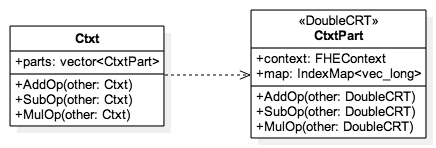
\includegraphics[width=0.65\textwidth]{CtxtTypeHierarchy.png}
\caption{HElib Type Hierarchy}
\label{fig:CtxtTypeHierarchy}
\end{figure}

Let $\ast$ be the operation being performed (here $\ast$ could stand for any of the operations, all of them are handled similarly) and $A$ and $B$ be the ciphertexts being operated on. The execution of the operation $ A = A\ \ast\  B$ requires a few steps. 

$A$ and $B$ are stored as \verb|Ctxt| objects in HElib. Figure \ref{fig:CtxtTypeHierarchy} shows the type hierarchy for a \verb|Ctxt| object. \verb|Ctxt| objects have one important variable, \verb|parts|, a vector containing multiple \verb|CtxtPart|s. These \verb|parts| constitute the ciphertext. The operations supported by \verb|Ctxt| are the addition, subtraction, and multiplication of two \verb|Ctxt| objects. Each of these operations use \verb|parts| during the execution of the operation, thus the operations in \verb|CtxtPart| are called.

\verb|CtxtPart| is an extension of the class \verb|DoubleCRT|, which is where the operations are implemented. Listing \ref{lst:HElibSerial} is an excerpt from the function that performs the operations.

\begin{lstlisting}[language=C++,caption={Add, Sub and Mul operations of two DoubleCRT objects},label={lst:HElibSerial}]
...
const IndexSet& s = map.getIndexSet();
long phim = context.zMStar.getPhiM();

for (long i = s.first(); i <= s.last(); i = s.next(i)) {
    long pi = context.ithPrime(i);
    vec_long& row = map[i];
    const vec_long& other_row = (*other_map)[i];

    for (long j = 0; j < phim; j++) {
      row[j] = fun.apply(row[j], other_row[j], pi);
    }
}
...
\end{lstlisting}

As the index set is iterated over, the i$^{th}$ prime is extracted along with the i$^{th}$ row from the maps. Even though the map is accessed like an array, it is an unordered map, with the array access syntax for convenience. These rows are then iterated over, applying the operation to each element. This is where the SIMD design is occurring, a double \verb|for| loop to add, subtract or multiply two vectors together. This is where the modifications and possible run time speedups can occur by using distributed system techniques.

\section{Distributed Systems}
Distributed systems is a field of computer science that deals with computer systems performing concurrent computation to achieve a goal. These systems can be as tight as a single computer running multiple threads or as loose as a group (cluster) of computers (nodes) connected via a message passing interface all over the world. What these systems have in common is that they are all connected and working to achieve a single goal.

The benefit of using a distributed computing system is the possibility for concurrent computation. Non-distributed computing systems are limited to only serial execution of programs. This means that if, for example, the system were tasked with adding two vectors together, it would have to loop over all entries one after the other and add each individually. For large vectors, this could be time consuming. Each individual operation is independent, and can therefore be performed at the same time. This is the purpose of a distributed system. By partitioning the data, and assigning a portion of the work to each node in the system, concurrent computation can be performed. For large vectors, this may result in a speedup in the run time, because of the concurrent execution.

The caveat of using a distributed computing system is the possibility for large overhead times, that can slow down computation. Time can be lost because of the added operations needed to facilitate the concurrent computation. The data must be partitioned and sent to the node that is performing the operation, which can cost time, if the means of transfer between nodes is slow, because in the original serial design, this did not occur. So for large vectors, it may be faster to perform the operation because of the concurrent execution, however in order to be able to perform the concurrent execution, some setup is required, that might cause the overall run time to be slower than the original serial execution. This is the trade off when working with distributed systems. Much work is done to reduce the amount of overhead in distributed systems, but they all suffer from it.

Distributed systems can be classified into two categories: parallel computing or distributed computing. A parallel computing system allows for shared memory, meaning that the processors all have access to a common memory which can be used to exchange information between processes. A common example of parallel computing is a graphics processing unit (GPU), because it is a single piece of hardware that has a common memory with many processors operating at once. In distributed computing systems, each processor has private memory and a message passing interface is used to exchange information between processes. A common example of this is the internet. Each computer attached to the internet has its own private memory and uses message passing to communicate with other machines on the internet. A common message passing interface is OpenMPI, which allows for the creation and running of a distributed computing system.

\subsection{Parallel Computing on GPU}
GPUs were designed to manipulate images for output on a display. Because of this, their design was such that they would perform operation in parallel over every pixel needing to be manipulated. Each pixel, or piece of data, was given its own compute core, that could be executed concurrently with every other compute core, which is how parallel execution was achieved. Expanding beyond manipulating images, one can see that this approach to computation can be applied to any circuit where the input is discrete and the same operation is applied to each piece of the input. 

Going back to the example given earlier, each element in the vectors can be assigned to a separate core. Then each core can be executed simultaneously, and the result will be generated. For large vectors, a loop's run time would increase as the size of the vector increased. However, by using a GPU, the run time would be the same for any size vector (because the operation being performed was always the same, and because all the cores were executed at the same time). It makes no difference if 20 or 20,000 cores were executed, they would both take the same amount of time. This has allowed GPUs to be used for many more purposes than just manipulating images, and in recent years to help speedup the run times of SIMD algorithms.

\subsection{Distributed Computing with OpenMPI}
Distributed computing systems are a cluster of machines all linked through a message passing interface. One would use a distributed computing system when computation can not be performed on a single system alone because either the input is too large or the computation will take too long. By partitioning the input and assigning each node a portion of the work, the task can be completed, where before it could not.

A widely used message passing interface is OpenMPI. OpenMPI allows for the creation of a distributed cluster with a single call, and provides functions to send and receive data from other nodes in the cluster easily. This allows for the partitioning and scheduling of work on a distributed system to be easily achieved.

Again addressing the example given earlier, depending on the number of nodes in the cluster, the vector can be partitioned so that each node gets roughly the same amount of elements. Each node can then compute the addition operation on only the portion of the vectors it is assigned. This allows for the concurrent execution of the addition operation, thus decreasing the run time compared to the serial computation. Distributed computing systems have become the design used by online services in recent years because they can service multiple customers at a single time, which is a desired feature when working on the internet.